\graphicspath{{chapters/04/media/}}
\chapter{Analisi dei dati}
\label{cha:analisi}
%  \begin{figure}[H]
%    \centering
%    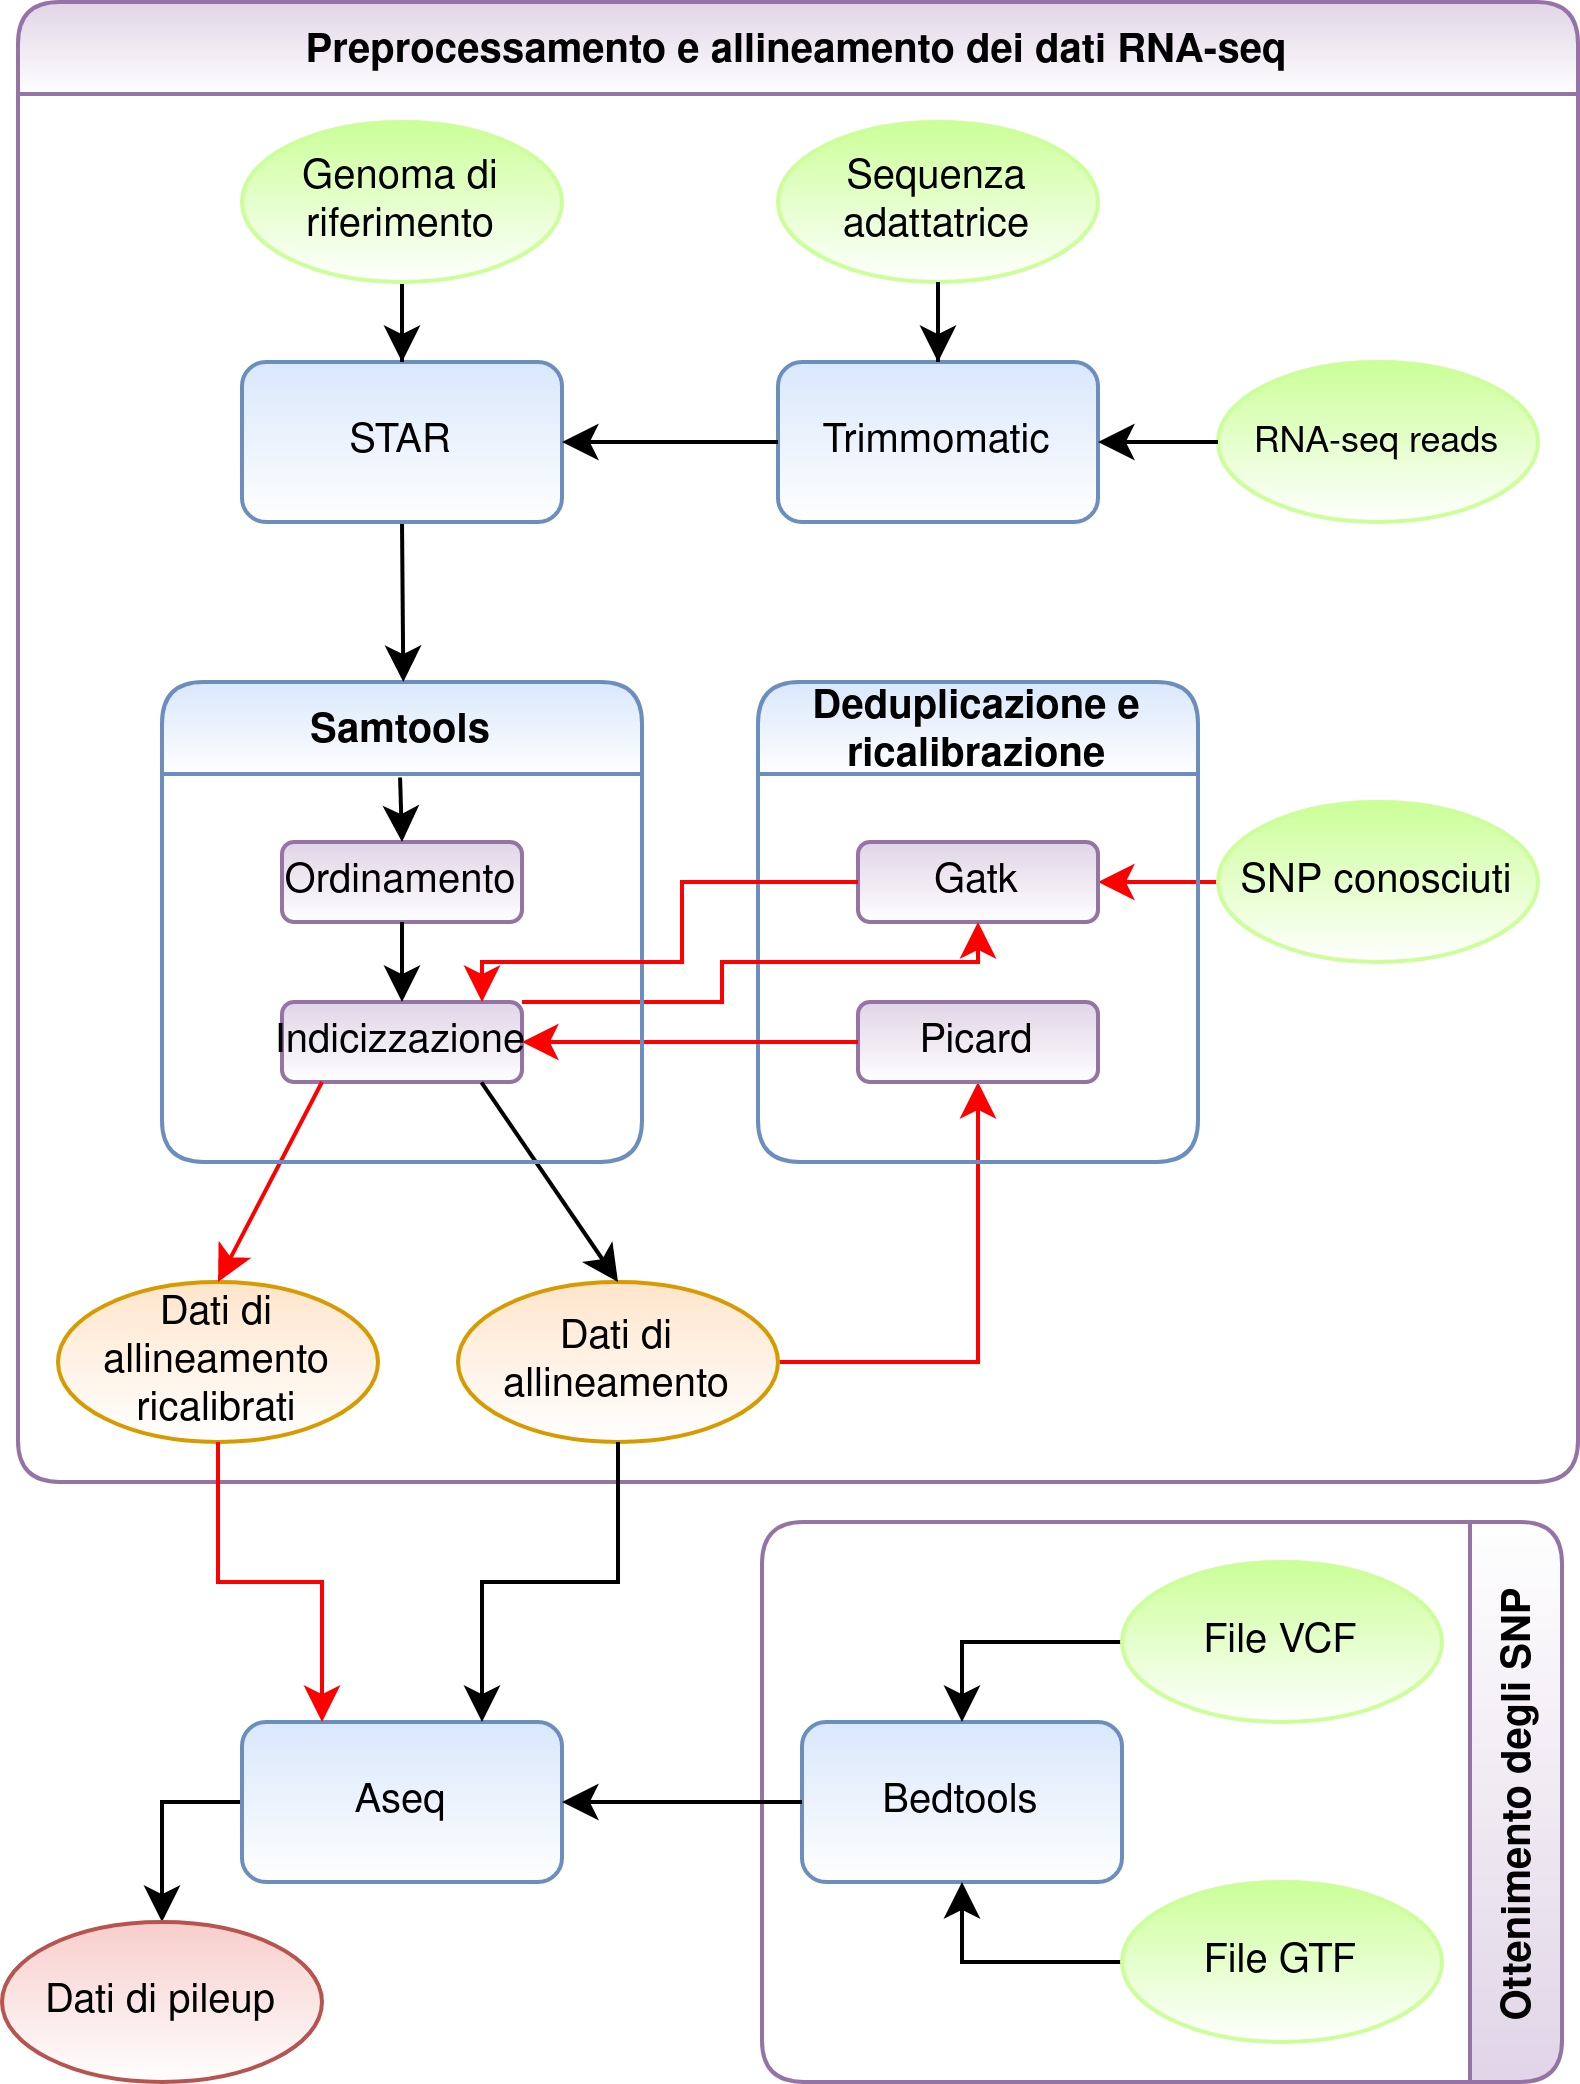
\includegraphics[scale=0.2]{pipeline.png}
%    \caption{Pipeline per l'ottenimento dei dati di allelic imbalance}
%    \label{fig:}
%  \end{figure}
\section{Conta degli SNP trovati con aseq}
\label{sec:snpcount}
Dall'esecuzione di aseq (\ref{sec:aseq}) si ottengono i valori di sbilanciamento allelico per tutti gli SNP ottenuti.
Seguendo le ``best practices'' di Gatk \cite{gatk} l'analisi \`e stata eseguita sui risultati di aseq ottenuti a partire dall'insieme dei file di allineamento generati dal processo di deduplicazione e ricalibrazione (\ref{subsec:deduprecal}).\\
Volendo considerare unicamente gli SNP presenti in eterozigosi i risultati sono filtrati considerando SNP con frazione allelica compresa tra $0.2$ e $0.8$.
Inoltre per aumentare il grado di confidenza dei risultati sono stati considerati unicamente gli SNP con un coverage\footnote{Si intende per coverage il numero medio di reads che coprono una regione genomica obiettivo} maggiore di $10$.
Queste due operazioni di filtraggio hanno portato all'identificazione di $20895$ SNP unici, $587$ dei quali condivisi tra tutte le condizioni e replicati.\\
Come aspettato la frazione allelica degli SNP cos\`i trovati \`e distribuita secondo una normale con la media centrata a $0.5$.\\
 \begin{figure}[H]
   \centering
   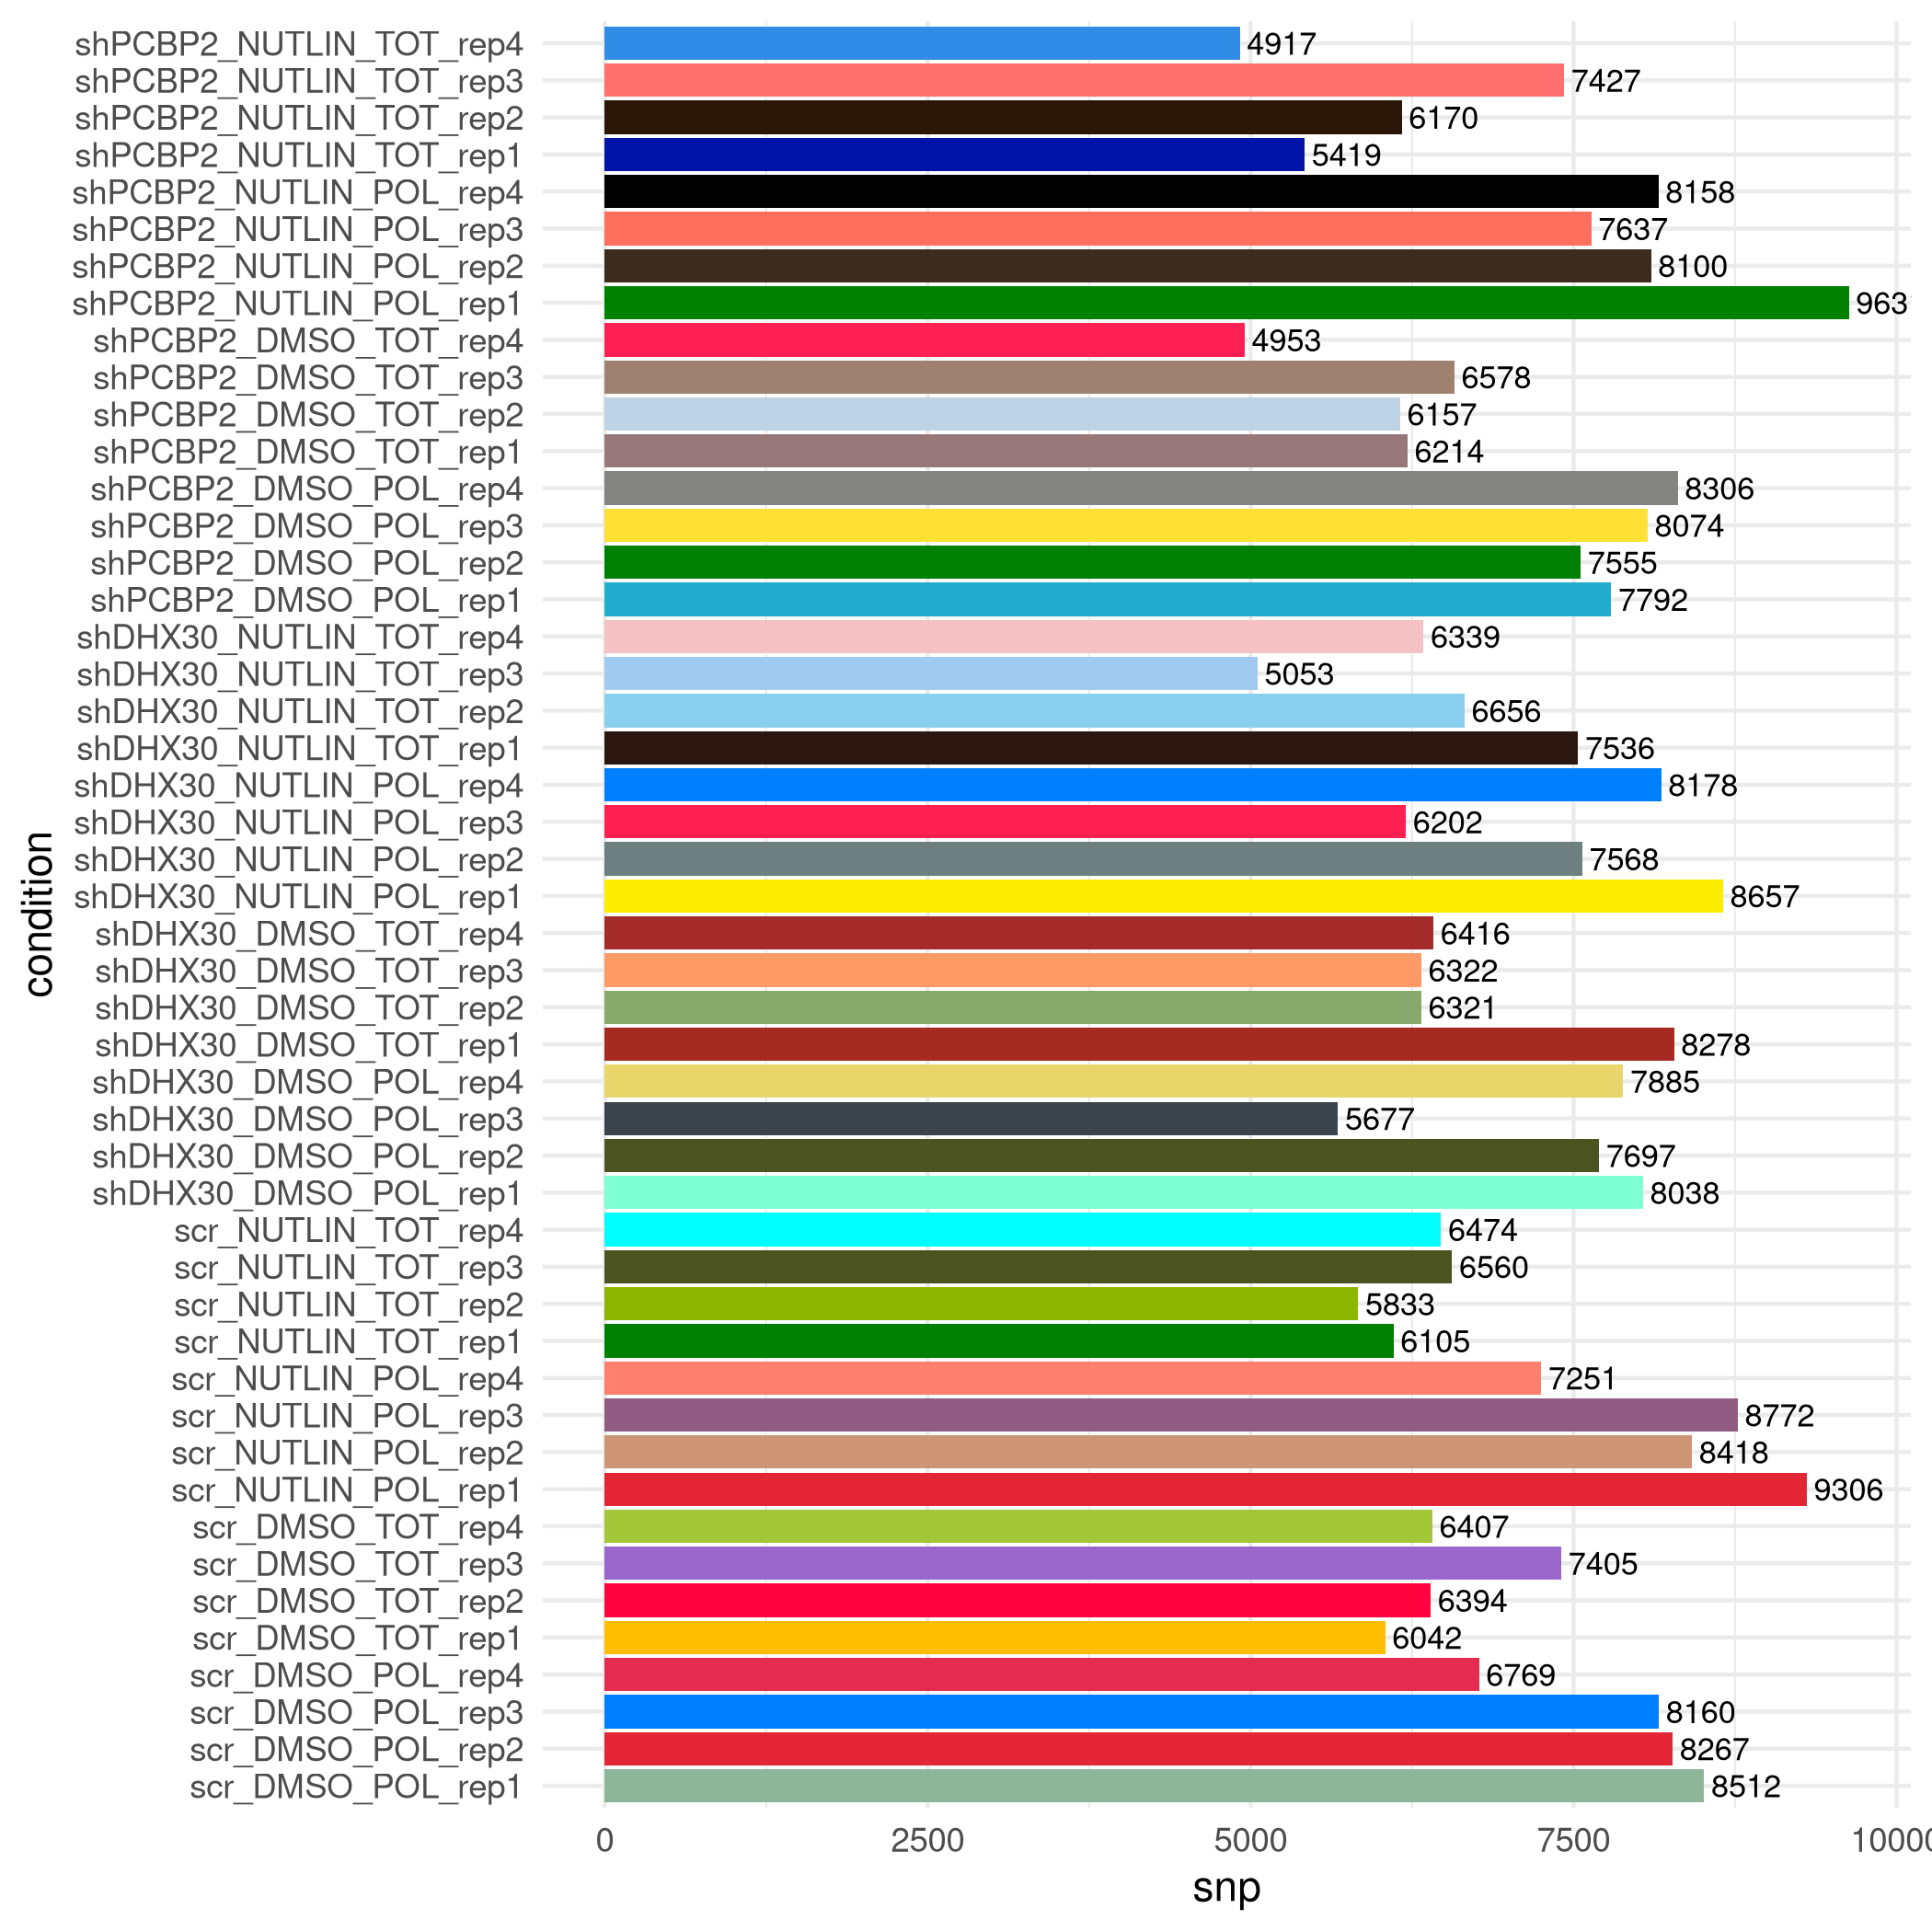
\includegraphics[scale=1]{aseq_count_2_8_10_pre.png}
	 \caption{Conta per campione degli SNP eterozigoti trovati con aseq ($0.2< af < 0.8$ e coverage $\ge 10$)}
   \label{fig:}
 \end{figure}

\section{Identificare gli SNP di interesse}
\label{sec:snp_filter}
La lista di SNP ottenuta dall'operazione di filtraggio dei risultati di aseq (\ref{sec:snpcount}) \`e stata ulteriormente confrontata con dati ottenuti da cellminer \cite{cellminer}.
Quest'ultima contiene $13681$ SNP gi\`a determinati come eterozigoti in HCT116.
A partire dalla lista sono stati raccolti i dati di tutti gli SNP che rispettano le condizioni di coverage e frazione allelica in almeno $3$ replicati biologici dei $4$ per condizione.
Questo viene fatto per dare forza statistica ai risultati e ridurre il rumore dovuto a errori nati dalla pipeline di analisi o alla variabilit\`a sperimentale della procedura di RNA-seq.\\
Per ognuno di questi SNP \`e stato svolto un t-test \cite{ttest} tra i valori di frazione allelica polisomiale e totale.
Sono stati infine considerati significativi gli SNP con p-value nominale risultato dal t-test inferiore a $0.05$.\\
Come si nota dalla tabella \ref{tab:significativesnp} gli SNP significativi trovati sono $161$, dei quali $60$ nella $3'$-UTR e $8$ nella $5'$-UTR.
\begin{table}[H]
	\begin{tabular}{|c|c|c|c|}
		\hline
		Condizione & Totali & $3'$-UTR & $5'$-UTR\\
		\hline
		scr\_DMSO & $27$ & $8$ & $2$\\
		\hline
		scr\_NUTLIN & $33$ & $11$ & $2$\\
		\hline
		shDHX30\_DMSO & $22$ & $9$ & $1$\\
		\hline
		shDHX30\_NUTLIN & $25$ & $11$ & $0$\\
		\hline
		shPCBP2\_DMSO & $24$ & $10$ & $1$\\
		\hline
		shPCBP2\_NUTLIN & $30$ & $11$ & $2$\\
		\hline
	\end{tabular}
	\centering
	\caption{SNP significativi per condizione}
	\label{tab:significativesnp}
\end{table}

\section{Caratterizzazione degli SNP di interesse}
L'ultimo passo dell'analisi \`e stata l'annotazione degli SNP in modo da determinare quali geni subiscono un cambio nel potenziale di traduzione causato da tali SNP.
L'annotazione \`e stata svolta grazie al tool snpEff \cite{snpeff}.
Confrontando i risultati dell'annotazione con una lista di geni coinvolti in molti tipi di cancro noti in letteratura si sono notati $14$ SNP che causano una variazione del potenziale di traduzione in $12$ geni.
In particolare $3$ di questi si trovano nella $3'$-UTR: \emph{rs788023} per il gene \emph{SF3B1}, \emph{rs30386} per \emph{TBC1D9B} e \emph{rs11539713} per \emph{KIF5B}.
La loro differenza nella frazione polisomiale e totale \`e descritta nei boxplot \ref{fig:SF3B1}, \ref{fig:TBC1D9B} e \ref{fig:KIF5B}.
\begin{multicols}{2}
\begin{figure}[H]
  \centering
  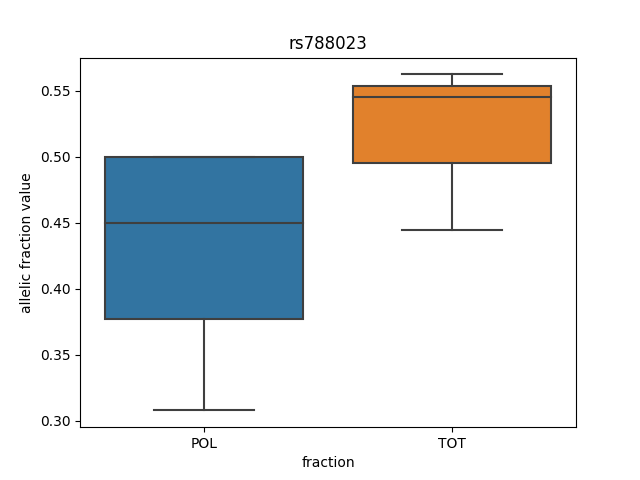
\includegraphics[scale=0.5]{scr_NUTLIN_rs788023.png}
  \caption{Variazione di sbilanciamento allelico tra frazione polisomiale e totale di rs788023 (p-value $0.0487$)}
  \label{fig:SF3B1}
\end{figure}

\begin{figure}[H]
  \centering
  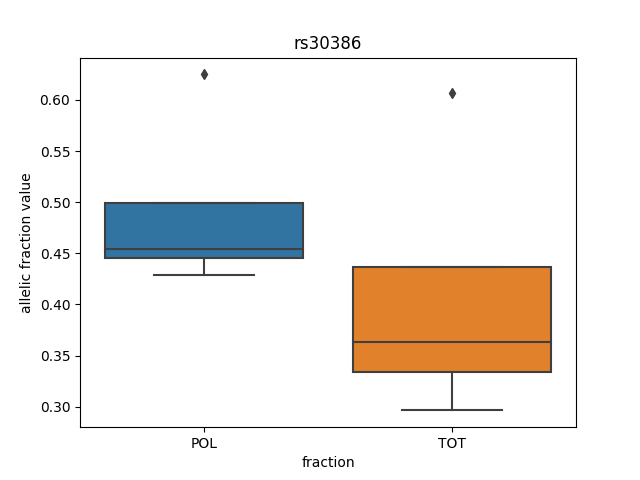
\includegraphics[scale=0.5]{scr_NUTLIN_rs30386.png}
  \caption{Variazione di sbilanciamento allelico tra frazione polisomiale e totale di rs30386 (p-value $0.0424$)}
  \label{fig:TBC1D9B}
\end{figure}

\begin{figure}[H]
  \centering
  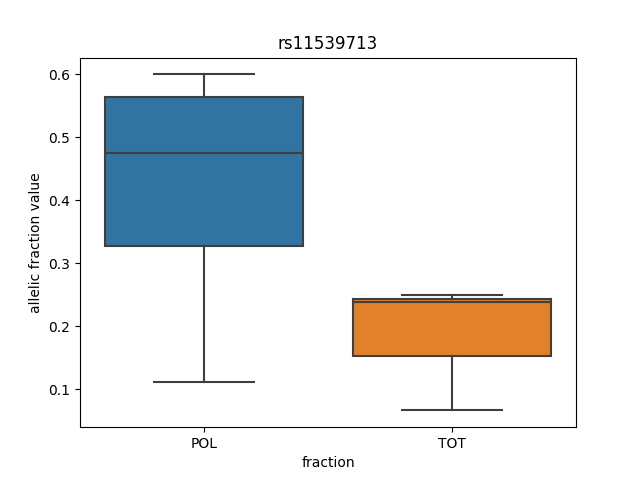
\includegraphics[scale=0.5]{shDHX30_DMSO_rs11539713.png}
  \caption{Variazione di sbilanciamento allelico tra frazione polisomiale e totale di rs11539713 (p-value $0.00099$)}
  \label{fig:KIF5B}
\end{figure}

\end{multicols}

	\subsection{SF3B1}
	Lo sbilanciamento nell'espressione traduzionale del gene SF3B1 si verifica in presenza di Nutlin e con stato genetico normale.
	Descritto in \cite{sf3b1}, questo gene codifica la subunit\`a $1$ del complesso proteico fattore di splicing 3b che insieme al fattore di splicing 3a e all'unit\`a a $12S$ RNA forma il complesso ribonucleoproteico piccolo o U2 snRNP.
	Il fattore di splicing 3b si lega al pre-mRNA a monte del sito intronico di ramificazione in maniera indipendente dalla sequenza e pu\`o ancorare U2 al pre-mRNA.
	Sue mutazioni sono state associate con diverse sindromi mielodisplasiche e altri tumori maligni ematologici, cancro al seno e melanoma uveale.
	Tipicamente \`e associato con dei sottotipi di sindromi mielodisplasiche caratterizzati da sideroblasti ad anello.

	\subsection{TBC1D9B}
	Lo sbilanciamento nell'espressione traduzionale del gene TBC1D9B (TBC1 domain family member 9b) si verifica in presenza di Nutlin e con stato genetico normale.
	Descritto in \cite{tbc1d9b}, questo gene codifica una proteina legante lo ione calcio e ha funzione come attivatore di GTPasi.
	Lo studio \cite{atf8} mostra come la proteina cos\`i prodotta interagisca con ATG8, regolando la formazione del trafficking degli autofagosomi.
	In particolare la sua capacit\`a di disattivare RAB11A facilita l'arrivo degli autofagosomi alla degradazione.

	\subsection{KIF5B}
	Lo sbilanciamento nell'espressione traduzionale del gene KIF5B si verifica in assenza di Nutlin e con knockdown di DHX30.
	Descritto in \cite{kif5b}, questo gene codifica una proteina motrice dipendente dai microtubuli necessaria per la distribuzione normale di mitocondri e lisosomi.
	Regola inoltre il posizionamento del nucleo e dei centrosomi durante l'inizio della mitosi.
	Oltre a ci\`o guida la separazione dei nuclei e dei centrosomi durante la fase $G2$.
	\`E anche in grado di guidare il movimento dei lisosomi verso la terminazione positiva dei microtubuli.
	Infine guida la polarizzazione dei granuli citolitici e dei centri organizzatori dei microtubuli.

\section{Conclusioni}
\label{sec:ending}
Il progetto presentato in questo elaborato sfrutta la grande quantit\`a di dati messa a disposizione dal next-generation sequencing per identificare e analizzare SNP che hanno possibili effetti nella regolazione traduzionale dei geni che li contengono nell’ambito del cancro. 
Dei $161$ SNP candidati identificati dall'analisi per HCT116, $60$ sono presenti nelle sequenze trascritte e non tradotte (UTR).
Tre di questi SNP potrebbero modulare l'efficienza traduzionale di $3$ geni coinvolti nello sviluppo e progressione tumorale.
Grazie all’analisi della regolazione traduzionale \`e possibile identificare meccanismi di regolazione prima non esplorati, aiutando a determinare quei processi cellulari alla base di eventi evoluzione tumorale, l'identificazione di marker prognostici o di resistenza alle terapie.
L'analisi, inoltre, evidenzia come Nutlin abbia un ruolo importante nel mettere alla luce questi eventi e come DHX30 sia coinvolta nel processo di regolazione traduzionale dei geni identificati. 
Questi geni potrebbero aiutare a scoprire i motivi dietro alle differenze di risposta a Nutlin di diversi tipi di cancro, permettendo un utilizzo mirato della molecola in ambito clinico e l'identificazione di nuove molecole attive contro specifici sottotipi tumorali.
L'identificazione di varianti ASE permette di generare ipotesi sui meccanismi molecolari coinvolti nell'evoluzione di specifici sottotipi tumorali, nell'aggressivit\`a e nell'evoluzione delle resistenze alle terapie che, se validate, permettono di approfondire il ruolo di specifici geni nel contesto tumorale. 
